\documentclass[12pt,english]{article}
\usepackage[affil-it]{authblk}
\usepackage{graphicx}
\usepackage[space]{grffile}
\usepackage{latexsym}
\usepackage{textcomp}
\usepackage{longtable}
\usepackage[flushleft]{threeparttable} 
\usepackage{multirow,booktabs}
\usepackage{amsfonts,amsmath,amssymb}
\usepackage{url}
\usepackage[utf8]{inputenc}
\usepackage{hyperref}
\hypersetup{colorlinks=false,pdfborder={0 0 0}}
%\usepackage{latexml}
\newcommand{\truncateit}[1]{\truncate{0.8\textwidth}{#1}}
\newcommand{\scititle}[1]{\title[\truncateit{#1}]{#1}}
%\usepackage{lmodern}
\usepackage[T1]{fontenc}
%\usepackage[latin9]{inputenc}
%\pagenumbering{gobble}

\providecommand{\tabularnewline}{\\}
\usepackage[nolist]{acronym}
\newacro{BMI} {body mass index}  
\newacro{LMICs} {low- and middle-income countries}  
\newacro{LMIC} {low- and middle-income country}  
\newacro{MICs} {middle-income countries} 
\acrodefplural{HIC}[HICs]{high-income countries}
\newacro{MIC} {middle-income country}  
\newacro{HIC} {high-income country}  
 \newacro{FE} {fixed effects}  
\newacro{HbA1c} {glycated hemoglobin}  
\newacro{IDF} {International Diabetes Federation}  
\newacro{IV} {instrumental variable}  
\newacro{LPM} {linear probability model}  
\newacro{MxFLS} {Mexican Family Life Survey}  
\newacro{OLS} {ordinary least squares}  
\newacro{RE} {random effects}  
\newacro{US} {United States}
\newacro{WHO} {World Health Organization} 
\newacro{USA} {United States of America}   
\usepackage{longtable}
\usepackage{booktabs}
\usepackage{multirow}
\usepackage{graphicx}
\usepackage[Export]{adjustbox}
%\newcommand{\sym}[1]{\ensuremath{^{#1}}} % for symbols in Table
%landscape pages
\usepackage{pdflscape}
\newcommand{\comment}[1]{}  %allows multiline comments
\usepackage[english]{babel}% Recommended
%\usepackage{csquotes}
\usepackage[
maxcitenames=2, 
style=authoryear-comp,
firstinits=true,
maxbibnames=99,
backend=biber,
uniquename=false,
url=false,
isbn=false]{biblatex}
\DeclareNameAlias{sortname}{last-first}
\DeclareFieldFormat{pages}{#1}%
\renewcommand*{\nameyeardelim}{\addcomma\space} %adds comma between name and years in citations

\renewbibmacro{in:}{}
\renewbibmacro*{volume+number+eid}{%
  \printfield{volume}%
  \setunit*{\adddot}% DELETED
  \setunit*{\addnbspace}% NEW (optional); there's also \addnbthinspace
 \printfield{number}%
 \setunit{\addcomma\space}%
 \printfield{eid}}
\DeclareFieldFormat[article]{number}{\mkbibparens{#1}}
\DeclareLanguageMapping{english}{english-apa}  %needed for APA style
\AtEveryBibitem{
  \clearfield{labelmonth}
}

\DeclareCiteCommand{\fullcite}
  {\usebibmacro{prenote}}
  {\usedriver
     {\defcounter{minnames}{6}%
      \defcounter{maxnames}{6}}
     {\thefield{entrytype}}.}
  {\multicitedelim}
  {\usebibmacro{postnote}}
%\addbibresource{/home/till/Dokumente/BibTex/Second_Mexico_paper-Article.bib}
\addbibresource{/home/till/Dokumente/BibTex/Thesis.bib}
%\usepackage[authoryear]{natbib}


% paper margins
\usepackage{geometry}
\geometry{
letterpaper,
left=25mm,
right=30mm,
top=20mm,
bottom=30mm,
}   
%limiting tables to only float within section
\usepackage{placeins}
  
%use for commands only working with pdf
  
% formatation

\usepackage{listings}
\lstset{ %
  backgroundcolor=\color{white},   % choose the background color
  basicstyle=\footnotesize,        % size of fonts used for the code
  breaklines=true,                 % automatic line breaking only at whitespace
  captionpos=b,                    % sets the caption-position to bottom
  commentstyle=\color{OliveGreen},    % comment style
  keywordstyle=\color{BlueViolet},       % keyword style
  stringstyle=\color{black},     % string literal style
  language=[AlLaTeX]TeX,             % Set your language (you can change the language for each code-block optionally)
  frame=lrtb, %
  xleftmargin=\fboxsep, %
  xrightmargin=-\fboxsep, %
  moretexcs={lstset,color,colorlet, cellcolor, newcolumntype, columncolor, rowcolor, multirow, xspace, LaTeX, TeX},
}

	% *****************************************************************
	% siunitx
	% *****************************************************************
	\usepackage{siunitx} % centering in tables
		\sisetup{
			detect-mode,
			tight-spacing		= true,
			group-digits		= false ,
			input-signs		= ,
			input-symbols		= ( ) [ ] - + *,
			input-open-uncertainty	= ,
			input-close-uncertainty	= ,
			table-align-text-post	= false
	        }
\usepackage[firstpage]{draftwatermark}	        
\begin{document}
\title{The impact of diabetes on labor market outcomes in Mexico: a panel data and biomarker analysis\thanks{Till Seuring is a post-doctoral researcher at the Leibniz Institute for Prevention Research and Epidemiology - BIPS and his email is seuring@leibniz-bips.de,  Pieter Serneels is Associate Professor at University of East Anglia and can be contacted at p.serneels@uea.ac.uk, Marc Suhrcke is Professor at the University of York and his email is marc.suhrcke@york.ac.uk.}}

\author[1,2]{Till Seuring%
	\thanks{Corresponding author}}
\author[2]{Pieter Serneels}
\author[3]{Marc Suhrcke}

\affil[1]{Leibniz Institute for Prevention Research and Epidemiology - BIPS}
\affil[2]{University of East Anglia}
\affil[3]{University of York}





\maketitle 
\begin{abstract}
Diabetes has become one of the most common chronic diseases in middle- and high-income countries. Yet, our understanding of its economic consequences remains limited. Making use of rich panel data for Mexico, where diabetes is the number one cause of death, we find evidence for adverse effects of self-reported diabetes on the probability of being employed, but not on wages or hours worked, using fixed effects estimation. Self-reported diabetes reduces the probability of employment with 5 percentage points for men and close to 6 percentage points for women.  Considering different types of work, the relationship between self-reported diabetes, and wages and hours worked remains weak, but the results also suggest occupational selection with women with self-reported diabetes less likely to work in agriculture.  A dynamic analysis finds that the employment probability falls gradually over the years after having been diagnosed with this chronic condition.  Using unique biomarker data for a large subsample, we find that two thirds of those tested positive do not self-report diabetes, while 19\% of those who self-report have levels below the clinical threshold.  We contrast the impact of self-reported and tested diabetes, and find that it is similar for women but not for men.  Combined results suggest lower employment for those self-reporting, especially for men, while there is no employment effect for undiagnosed men or women, who tested positive but did not self-report.  This lack of employment effect for undiagnosed men seems to stem from better general health rather than less severe diabetes. The results highlight both the importance of the economic impact of diabetes, and the need to take into account (especially female) undiagnosed patients.
\end{abstract}



\section{\label{sec:Introduction4}Introduction }

Diabetes, and particularly its most common variant, type 2 diabetes, has increased worldwide and is expected to continue to rise over the next decades \parencite{Risk2016}. The condition has become a problem for middle-income countries and high-income countries alike, with over two-thirds of people with diabetes living in the developing world \parencite{InternationalDiabetesFederation2013}. Mexicans and Mexican-Americans appear to be particularly affected by diabetes, also in comparison to other Latino populations living in the USA \parencite{Schneiderman2014}. In Mexico itself, diabetes prevalence has been estimated to have grown from 6.7\% in 1994 to 14.4\% in 2006, including both diagnosed and undiagnosed cases \parencite{Barquera2013}, and is expected to increase further over the next decades \parencite{Meza2015}. Already now, diabetes is the number one cause of death in Mexico \parencite{Barquera2013}. 

The observed trend has been attributed to a deterioration in diet and a reduction in physical activity \parencite{Barquera2008b,Basu2013}, while genetic predisposition among Mexicans with pre-hispanic ancestry may also play a role \parencite{Williams2013}. Recent evidence indicates that the onset of diabetes has been occurring at an ever earlier age in Mexico \parencite{Villalpando2010}. With treatment as ineffective as it currently is---only a minority achieves adequate blood glucose control \parencite{Barquera2013}---the earlier start will increase the likelihood of complications during the productive lifespan. 

Diabetes is a term used to describe various conditions characterized by high blood glucose values, with the predominant disease being type 2 diabetes accounting for about 90\% of all diabetes cases \parencite{Sicree2009}. The elevated
blood glucose levels that are a result of the body's inability to use insulin properly to maintain blood glucose at normal levels, can entail a range of adverse health effects for the individual concerned. However, via effective self-management of the disease much if not all of the complications can be avoided \parencite{Lim2011, Gregg2012}. In the absence of this management---or in the case of inadequate treatment---diabetes has been documented to lead to conditions such as heart disease and stroke, blindness, kidney problems, and nerve problems which together with impaired wound healing can lead to the loss of limbs \parencite{Reynoso-Noveron2011}. These conditions can be seriously debilitating and may therefore reduce an individual's economic activity, including its productivity and labor market participation.

The effect of diabetes on labor outcomes has been studied predominantly in high-income countries where diabetes has been found to be associated with reductions in employment probabilities as well as wages and labor supply \parencite{Brown2005,Brown2014,BrownIII2011,Minor2011,Minor2013,Minor2015,Latif2009,Seuring2015a}.\footnote{We know of only two studies for middle income countries, one for Mexico \parencite{Seuring2015} and one for China \parencite{Liu2014}, which are discussed later in more detail.}

While these studies have provided useful evidence , many of the complexities of the relationship between diabetes and labor outcomes remain have remained unaddressed. Unobserved heterogeneity presents a challenge when estimating the relationship between diabetes and labor outcomes. Especially time-invariant unobserved individual characteristics, like health endowments , as well as risk preferences have been shown to adversely affect health in general and the propensity to develop type 2 diabetes more specifically \parencite{VanEwijk2011,Sotomayor2013,Li2010b}; they may also affect employment probabilities, wages or working hours---either directly through their effects on contemporaneous productivity \parencite{Currie2013} or indirectly by limiting educational attainment and human capital accumulation \parencite{Ayyagari2011a}. Further, given the chronic nature of the condition, it would be of interest to better understand when potential labor market penalties appear, and how these effects change over time. 

Finally, given that most studies rely on self-reported diabetes data, it is of interest to contrast estimates obtained from this data with those yielded from clinical test data on diabetes. Especially in a middle income country setting, where large parts of the population remain undiagnosed, this can reveal hidden impacts, namely for those who are unaware of the disease. Diabetes may also have an effect in itself. People aware of their condition may, for instance, be less inclined to continue working if this interferes with their disease management, they may be suffering from psychological stress, depression, or anxiety, because of becoming aware of the disease; they may also use the diagnosis as a justification for decreasing their labor supply \parencite{Kapteyn2009}. As a consequence labor market effects may be distinct for people with self-reported versus those unaware of their condition, potentially leading to biased estimates if the analysis is based on self-reports alone.

The objective of this study is to provide new evidence on the impact of diabetes on labor outcomes, and improve upon previous work by paying close attention to the above challenges. We use three waves of panel data from the \acf{MxFLS}, covering the period 2002--2012. The \ac{MxFLS} is particularly useful for the analysis of diabetes as it allows accounting for the above complexities in more refined ways than existing studies. Using individual level \acf{FE} analysis for the first time in this literature, we take account of time-invariant heterogeneity when assessing the impact of self-reported diabetes and its duration on labor outcomes.\footnote{A recent review of the economic cost of diabetes confirms the scarcity of evidence for low- and middle-income countries \parencite{Seuring2015a}.}  Using novel and rich biomarker data we also explore the role of undiagnosed diabetes---an issue of considerable importance in light of its high prevalence (see \textcite{Beagley2014}) and because it has remained unaccounted for in most earlier studies, which typically rely on self-reported information. Doing so sheds light on the issue of measurement error and the potentially differential effects of self-reported and undiagnosed diabetes.

Our results using self-reported diabetes suggest an economically important decrease in the employment probability of people aware of their disease. Wages and working hours, however, do not appear to be lower for those with self-reported diabetes. A dynamic analysis indicates that employment probabilities are reduced gradually with each additional year since diagnosis, with some evidence for an even larger effect per year after the initial 10 years.

The biomarker analysis indicates that clinically diagnosed diabetes entails a significant employment penalty for women but not for men. Assessing the effects of both clinical and self-reported diabetes at the same time provides an insight into the labor market impact for those with undiagnosed diabetes---people who are tested positive but did not self-report. The results suggest that self-reporting in itself has a negative and significant effect for men, but the effect is not statistically significant for women, possibly  due to large standard errors. In contrast we find no evidence for an effect of undiagnosed diabetes. 


\section{\label{sec:labor  outcomes and diabetes literature}Diabetes and labor outcomes---what do we know?}

A limited number of studies provides insights on the relationship between diabetes and labor outcomes.  Table 1 in appendix summarises the main findings of these studies, the characteristics of the sample and estimation method they use, and the approach to measure diabetes.  To the best of our knowledge only two studies exist for developing countries. \textcite{Liu2014} exploiting a natural experiment in China, find a significant reduction in income for those with a recent diagnosis of diabetes. A study for Mexico using cross-section data from 2005, finds a significant (p<0.01) reduction in employment probabilities for males by about 10 percentage points and for females by about 4.5 percentage points (p<0.1), using parental diabetes as an \ac{IV} \parencite{Seuring2015}.

A small number of studies have investigated the effects of diabetes on labor outcomes in high income countries. \textcite{Brown2005} consider an elderly population of Mexican Americans living in the US, close to the Mexican border, and find a significant adverse relationship, with 7 percentage points lower employment rates for men with self-reported diabetes, while for women, the negative relationship becomes insignificant when using \ac{IV} estimation.  In a similar vein , \textcite{BrownIII2011}, again considering a cross-section of Mexican-Americans,  find a negative  relationship between the level of \ac{HbA1c} and the probability of employment as well as the wage for men, but not for women.  

Slightly different results are obtained in two other studies, this time for the USA in general. Using a sample comprised exclusively of women, \textcite{Minor2011} finds self-reported diabetes to have a significant negative effect on female employment and earnings but not on working hours. The study finds self-reported diabetes to be endogenous and estimates upward biased compared to \ac{IV} estimates. In a later study \textcite{Minor2013} finds that employment probabilities decline shortly after diagnosis for men and after about 10 years for women, while wages are not affected by the duration of the condition, using cross section data. 

As far as we know, only one paper considers undiagnosed diabetes. \textcite{Minor2015} finds a negative, but not statistically significant, relationship between undiagnosed diabetes and the probability of, in particular, female employment. They further find a negative and statistically significant relationship of self-reported diabetes with employment for both men and women. When combining both the undiagnosed and self-reporting, the relationship with employment remains statistically significant but becomes less negative. However, the results of this part of the study are based on a very small sample size.

Results for Canada indicate a significant negative impact of self-reported diabetes on the employment probability  for women, but not for men \parencite{Latif2009}, using an IV strategy similar to \textcite{Brown2005}, and suggesting diabetes to be  endogenous for men, resulting in upwards biased estimates,  but not for women. For Australia, \parencite{Zhang2009} find  reduced labor market participation for men and women as a result of diabetes, with the effects appearing overstated if the endogeneity of diabetes is unaccounted for.



While the above existing studies suggest that diabetes can impose substantial economic losses on individuals and households, most of these studies have one or more methodological limitations.  
Mostly using cross sectional data, they cannot account for unobserved characteristics.  As a result it often remains uncertain whether the estimated coefficient reflects  a causal relationship.  A number of papers try to address this bias, typically using the family history of diabetes as identifying instrument. This relies on the genetic and heritable component of type 2 diabetes but it remains unclear whether the variable satisfies the exclusion restriction, as it may also proxy for other genetically transferred traits, including unobserved abilities, as well as  intrahousehold or intergenerational dynamics that impact labor outcomes directly.\footnote{It is conceivable that diabetes might deteriorate parental health in such a way that the offspring either has to give up their employment to provide care, or has to increase labor supply to compensate for lost income, as also argued by \textcite{Seuring2015}.} 

Furthermore, most---but not all---studies use self-reported diabetes as a proxy for diabetes. Self-reported health data can suffer from  several short comings, and introduce non-classical measurement error due to systematic misreporting. This has been shown to cause estimates of economic impacts to be potentially biased and overstated \parencite{Cawley2015,ONeill2013,Perks2015}.  In the context of diabetes, the concern is especially related to possible false negatives. False positives might be less of a problem since there seems to be limited incentive to report diabetes when one does not have it – although we cannot exclude this.  A recent study from China confirms that those who self-report diabetes are highly likely to actually have diabetes (>98\%), while only a minority of those who have diabetes (40\%) according to clinical tests, actually self-report the disease \parencite{Yuan2015}. This pattern is confirmed in our data where only a tiny proportion of the respondents reports to have diabetes while having biomarker results below the diabetes threshold. Of these, many likely have diabetes but treatment has pushed their \ac{HbA1c} levels back below the threshold, so that likely only very few respondents misreport their status.  However, a much larger proportion misreports to not have diabetes (18\%). The key concern thus lies with false negatives, as people may either have forgotten that they have been diagnosed with the condition, or have never been diagnosed.   These undiagnosed may have a distinct profile, they may for instance not be able to afford health care, live further away from a health facility,  or their diabetes has remained mostly asymptomatic so far.

This paper makes headway to overcome these key limitations in two ways, using a rich data set for Mexico.  First, it applies, making use of panel data, fixed effects estimation that allows controlling for unobserved time invariant characteristics.  Second, it makes use of biomarker data for a large subsample of the population. This allows us to carry out a comparison between the effect of self-reported and clinically tested diabetes. Given the careful measurement of self-reported diabetes in our case it also allows inference about the effects for undiagnosed patients, who suffer from diabetes according to a clinical test, but are unaware of this. To further our understanding of the relationship between diabetes and labor outcomes, we also consider its effect on the type and sector of employment, and the dynamic effects in the years after diagnosis.

\section{\label{sec:Data}Context and Data}

Mexico is a middle-income country with among the highest prevalences of obesity and diabetes in the world \parencite{InternationalDiabetesFederation2015,WHO}. A recent study showed that diabetes accounted for one-third of all deaths in a large sample of Mexicans 35 to 74 years of age in Mexico City, with renal disease, cardiac disease, infection, acute diabetic crisis, and other vascular diseases being the biggest contributors to the elevated mortality risk of people with diabetes \parencite{Alegre-Diaz2016}. The high disease burden of diabetes coexist with high levels of infectious diseases in Mexico, exposing the health system to a 'double-disease burden' that increases the pressure to identify treatment priorities and to efficiently use the existing resources, with the treatment of non-communicable diseases not being well integrated in the health care system \parencite{Gutierrez-delgado2009}. Earlier studies point to an underwhelming performance of the health system in diagnosing and effectively treating diabetes in Mexico, with most persons with diabetes achieving only poor glucose control and suffering from other untreated risk factors such as hypertension \parencite{Alegre-Diaz2016,Flores-Hernandez2015,Barquera2013}. Additionally, about half of the diabetes population has been estimated to be unaware of the condition \parencite{Barquera2013}.

This paper uses the \acf{MxFLS}, a nationally representative, longitudinal household survey which has three waves conducted in 2002, 2005--2006 and 2009--2012. All household members aged 15 and above were interviewed, covering information on a wide range of social, demographic, economic and health characteristics of the individuals and their families \parencite{Rubalcava2013}. Throughout the analysis the samples we use are restricted to the working age population (15--64). Our first part of the analysis uses all three waves, taking advantage of the large amount of observations and the panel structure of the data. The second part uses a biomarker subsample of the third wave (2009---2012). It is important to note that this sample is somewhat older on average, as it includes everybody above the age of 44 but only a random subsample of those aged 44 or below \parencite{Crimmins2015}. This also leads to self-reported diabetes being higher for this subsample. The biomarker analysis will therefore be compared for this subsample specifically.

The analysis focuses on the labor outcomes employment, hourly wage and weekly working hour, as well as occupation.\footnote{Employment status is defined as having worked or carried out an activity that helped with the household expenses the last week and working for at least four hours per week. We explicitly include those employed informally, for instance people working in a family business. We tested if changing the definition of being employed to having worked at least ten hours per week, and this only leads to marginal changes in the coefficients and standard errors, not affecting the interpretation of the results. Hourly wage was calculated by adding up the reported monthly income from the first and second job (if any) and dividing it by the average number of weeks per month providing us with an estimate of the average earnings per week, which is then divided by the weekly working hours to arrive at the hourly wage.  labor income was reported in two ways: either responding to questions on wages, income from piecework, tips, income from extra hours, meals, housing, transport, medical benefits and other earnings, or by reporting the aggregate labor income for the whole month. We adjusted the calculated wage for inflation from the year of the interview up to 2013 and consider the log of real wages.  Due to a considerable number of missing or zero income reports, the sample used for the wage estimation is smaller than the sample for working hours. Working hours reflect working hours of the first and second job (if applicable).}  About half of the respondents in the sample live in rural areas. Looking at our outcome variables, 86\% of men report some form of employment compared to 37\% of women. Interestingly, men do not report considerably higher hourly wages than women but work more hours per week. Also, men are working more often in agricultural jobs while women are more likely to be self-employed or in non-agricultural wage employment. Women also have lower educational attainment on average (see Table \ref{tab:Pooled-sample-characteristics}).

 


In the first part of the analysis we focus on the relationship of labor outcomes with self-reported diabetes \footnote{Self-reported diabetes is based on the survey question: “Have you ever been diagnosed with diabetes?”}, following the dominant approach in the literature. For the pooled data of all three waves (Table \ref{tab:Pooled-sample-characteristics}), diabetes was self-reported by 5\% of men and 6\% of women, respectively. This is consistent with \textcite{Barquera2013} who observe a prevalence of diagnosed diabetes in Mexico of 7.5\% in 2006, using a slightly older sample that also included elderly above the age of 64. Apart from self-reported diabetes information that is available in all rounds, we also use information on the self-reported year of diagnosis as well as biomarker data including \ac{HbA1c} levels for a subsample of respondents. 

Because self-reported diabetes reporting inhibited some inconsistency over time for some of the respondents, we tried to increase the consistency by using disease information from earlier and ensuing waves to infer on the current, missing or inconsistent, diabetes status. Appendix 1 provides details on the applied correction procedures. An further, and no less important, source of measurement error with self-reported diabetes is the omission of those with undiagnosed diabetes, i.e the false negatives. In order to investigate how this may affect estimates of the labor market impact of diabetes, we use information from a subsample of the 2009-2012 wave containing over 6000 respondents (everybody aged 45+ and a random subsample of those aged 15–44 (Crimmins et al., 2015)) that have biometrically measured blood glucose values, allowing for the identification of those with undiagnosed diabetes. Throughout, our analysis focuses on the working age population (15–64), and excludes pregnant women and those in school.\footnote{Pregnant women have an increased diabetes risk and this may bias the estimated impact of diabetes on female employment status. We dropped all observations of women reporting to be pregnant at the time of the survey (N=764).} Apart from self-reported diabetes information available in all waves, we also use information on the self-reported year of diagnosis---available in the third wave---to construct a measure of the time since diagnosis for all waves. Importantly, this limits the sample of the time since diagnosis analysis to those that were present in the third wave. 

\begin{table}[p]
\caption{\label{tab:Pooled-sample-characteristics}Descriptive statistics for panel and biomarker sample.}

\begin{adjustbox}{max width=\linewidth, center}
\begin{threeparttable}  %adds notes to tables
{
\def\sym#1{\ifmmode^{#1}\else\(^{#1}\)\fi}
\begin{tabular}{l*{4}{SS}}
\toprule
                    &\multicolumn{2}{c}{Panel}&\multicolumn{2}{c}{Biomarker}\\\cmidrule(lr){2-3}\cmidrule(lr){4-5}
                    &\multicolumn{1}{c}{Males}&\multicolumn{1}{c}{Females}&\multicolumn{1}{c}{Males}&\multicolumn{1}{c}{Females}\\
                    \midrule
\hspace*{10mm}\emph{Dependent variables} \\
Employed           &        0.86&        0.37&        0.86&        0.34\\
                    &      (0.34)&      (0.48)&      (0.35)&      (0.47)\\
Hourly wage (Mexican Peso)        &      42.47&       40.49&       36.30&       35.23\\
                    &    (485.87)&    (142.08)&     (53.69)&     (43.63)\\
Weekly working hours&      46.82&       38.99&       46.00&       38.15\\
                    &     (16.79)&     (18.90)&     (16.89)&     (19.65)\\
Agricultural worker &        0.22&        0.04&        0.25&        0.03\\
                    &      (0.41)&      (0.20)&      (0.43)&      (0.18)\\
Self-employed       &        0.19&        0.28&        0.21&        0.32\\
                    &      (0.39)&      (0.45)&      (0.41)&      (0.47)\\
Non-agricultural worker &&&&\\
or employee& 0.59&        0.68&        0.53&        0.64\\
                    &      (0.49)&      (0.47)&      (0.50)&      (0.48)\\
\hspace*{10mm}\emph{Diabetes variables} \\
Self-reported diabetes  &         0.05&        0.06&        0.09&        0.12\\
                    &      (0.22)&      (0.24)&      (0.29)&      (0.32)\\
Diabetes duration if self- &&&&\\
reported diabetes (years)   &        7.49&        7.83&        7.48&        7.99\\
                    &      (6.01)&      (7.83)&      (6.07)&      (7.03)\\
Glycated hemoglobin (HbA1c)&            &            &       6.46&        6.58\\
                    &            &            &      (1.89)&      (2.02)\\
HbA1c $\geq 6.5\%$  &            &            &        0.26&        0.28\\
                    &            &            &      (0.44)&      (0.45)\\
Undiagnosed diabetes&            &            &        0.18&        0.18\\
                    &            &            &      (0.39)&      (0.39)\\
\hspace*{10mm}\emph{Education and demographic variables} \\
Age                 &       36.03&       36.29&       42.78&       42.79\\
                    &     (13.62)&     (13.17)&     (14.28)&     (13.94)\\
Rural village of < 2,500&        0.44&        0.43&        0.50&        0.46\\
                    &      (0.50)&      (0.50)&      (0.50)&      (0.50)\\
Married             &        0.54&        0.54&        0.60&        0.56\\
                    &      (0.50)&      (0.50)&      (0.49)&      (0.50)\\
Number of children (age < 6) &&&&\\
in household&        1.48&        1.57&        1.18&        1.22\\
                    &      (1.45)&      (1.47)&      (1.29)&      (1.32)\\
Indigenous group    &        0.19&        0.19&        0.19&        0.18\\
                    &      (0.39)&      (0.39)&      (0.39)&      (0.39)\\
Secondary           &        0.30&        0.30&        0.26&        0.26\\
                    &      (0.46)&      (0.46)&      (0.44)&      (0.44)\\
High school         &        0.16&        0.13&        0.14&        0.12\\
                    &      (0.36)&      (0.34)&      (0.34)&      (0.33)\\
Higher education    &        0.11&        0.09&        0.12&        0.09\\
                    &      (0.32)&      (0.29)&      (0.32)&      (0.28)\\
\midrule
Observations        &    21388&       27341&        2785&        3623\\
\bottomrule
\end{tabular}
\begin{tablenotes}
\item \footnotesize \textit{Notes} Mean values, standard deviations in parenthesis. Results for the other variables, i.e. the Mexican states and wealth, are omitted to save space.
\end{tablenotes}
}
\end{threeparttable}
\end{adjustbox}
\end{table}


The biomarker data suggest that a relatively large share of the population (27\%) have an \ac{HbA1c} indicative of diabetes, defined by the \ac{WHO} as levels equal to or above 6.5\% \parencite{WorldHealthOrganization2011}. As argued by others, these rates of elevated \ac{HbA1c} levels in Mexico are high when compared to \ac{HbA1c} data from similar surveys in the USA and China \textcite{Frankenberg2015}. 
A second striking observation is that  68\% of males and females who test positive do not self-report: they are unaware of their condition. This may mean that estimates based on self-reported diabetes as a measure for diabetes may be biased, and underlines the importance of comparing with estimates based biomarker analysis. 19\% of respondents who self-report, has levels below the clinical threshold, possibly because they have managed their disease, although we cannot exclude misreporting of diagnosis.
%\FloatBarrier

\section{\label{sec:Estimation Strategy}Estimation strategy}


\subsection{Panel data on self-reported diabetes}

To investigate the relationship between self-reported diabetes and three labor outcomes: employment, wages and weekly working hours, respectively, we estimate the following \acf{FE} model.\footnote{We also estimated random effects models and but do not present them here as the Hausman test suggested the use of the FE model throughout. The estimates also do not vary widely. Results are obtainable upon request.}


\noindent 
\begin{equation}
Y_{it}=\beta_{0}+\beta_{1}Diabetes_{it}+\beta_{2}X_{it}+c_{i}+\gamma_{t}+u_{it}.\label{eq:cha4_employed}
\end{equation}


where $Y_{it}$ is a binary variable taking a value of $1$ if respondent $i$ reports being in employment at time $t$ and $0$ otherwise, $Diabetes_{it}$ is a binary variable taking a value of $1$ at time $t$ if the respondent reports having ever received a diagnosis of diabetes\footnote{We are not able to distinguish between type 1 diabetes and type 2 diabetes using this data. Other studies that tried to assess the effect of type 1 diabetes on labor outcomes have found no association \parencite{Minor2011,Minor2015}. Including type 1 diabetes therefore likely attenuates any adverse relationship we may find.}, $X_{it}$ is a vector of control variables, $c_{i}$ represents an individual fixed effect, $\gamma_{t}$ represents year dummies, and $u_{it}$ is the error term.

For the relationship of self-reported diabetes with wages and working hours our empirical models are estimated conditional on being in employment, and $Y_{it}$ represents the log hourly wage or the weekly working hours over the last year, for respondent $i$ at time $t$.

The control variables in both \ac{FE} specifications include dummy variables to capture the effects of the living environment, of living in a small, medium or large city with rural as the reference category, and state dummies. We also include a marital status dummy and the number of children residing in the household below the age of 6 to control for the impact of marriage and children on labor outcomes and the effect of childbearing and related gestational diabetes on the probability of developing type 2 diabetes
\parencite{Bellamy2009}. To account for the effect of changes in household wealth on diabetes and employment probabilities, we use standard
principal component analysis of multiple indicators of household assets and housing conditions to create an indicator for household wealth \parencite{Filmer2001}\footnote{Our composite wealth index consists of owning a vehicle, a second house, a washing machine, dryer, stove, refrigerator or furniture, any electric appliances, any domestic appliances, a bicycle or farm animals. It further accounts for the physical condition of the house, proxied by the floor material of the house, and the type of water access.}. The models also include a quadratic age term and calendar year dummies to capture the non-linear effect of age and a time trend, respectively.

Note that while using individual level \ac{FE} does not allow to fully identify a causal relationship, it does improve considerably on existing estimates, which are typically obtained from cross-section analysis, or from \ac{IV} estimation which tend to be weakly identified.  The FE model does control for unobserved personal characteristics, although time-variant omitted variables may still simultaneously drive labor and health. With respect to employment status, one potential concern could be that job loss affects lifestyle choices, which may increase the probability to develop diabetes, and could in turn negatively affect labor outcomes. Existing work for high income countries finds no evidence for reverse causality, as job loss does not seem to affect the probability to develop diabetes \parencite{Bergemann2011,Schaller2015}. Another possible channel might be that stress at work leads to a higher propensity of developing type 2 diabetes \parencite{Heraclides2012,Eriksson2013}. However, while stress levels may change over time, a person’s coping mechanisms to deal with stress are likely time-invariant \parencite{Schneiderman2005}. While we cannot exclude a role of time-variant unobserved factors, there seems to be consensus that time-invariant variables, including genetic predisposition and stable personality traits, may be more important. The \ac{FE} approach should then limit the bias resulting from these time-invariant confounding factors.


\subsection{Labor outcomes and time since diagnosis}

Given the chronic nature and irreversibility of diabetes, it is of interest to look at the dynamic effects after diagnosis.  We estimate the following model with years since self-reported diagnosis as the right hand side variable:

\begin{equation}
Y_{it}=\beta_{0}+\beta_{1}Dyears_{it}+\beta_{2}X_{it}+c_{i}+u_{it},\label{eq:duration_linear}
\end{equation}

\noindent where $\beta_{1}Dyears_{it}$ is a continuous variable indicating years since first reported diabetes diagnosis. To capture possible non-linearities in the relationship we then use a spline function that allows for the effect of an additional year with diabetes to vary over time.

\begin{equation}
Y_{it}=\delta_{0}+g(Dyears_{it})+\delta_{2}X_{it}+c_{i}+u_{it}.\label{eq:splines}
\end{equation}

\noindent with $g(Dyears_{it})=\sum_{n=1}^{N}\delta_{n}\cdot max\{Dyears_{it}-\eta_{n-1}\}I_{in}$ and $I_{in}=1[\eta_{n-1}\leq Dyears_{it}<\eta_{n}]$, with $\eta_{n}$ being the place of the $n$-th node for $n=1,2,\ldots,N$. We choose three nodes that---based on visual inspection---best captured any possible non-linearity in the
relationship between diabetes duration and labor outcomes, see Figures \ref{fig:Kernel-weighted-local-polynomial_empl}, \ref{fig:Kernel-weighted-local-polynomial_wage} and \ref{fig:Kernel-weighted-local-polynomial_workhrs} on pages \pageref{fig:Kernel-weighted-local-polynomial_empl}, \pageref{fig:Kernel-weighted-local-polynomial_wage} and \pageref{fig:Kernel-weighted-local-polynomial_workhrs}, respectively). These are located at 4, 11 and 20 years after diagnosis. The first four years should capture any immediate effects of the diagnosis, the years five to eleven should capture any effects of adaptation to the disease. After 11 years it is conceivable that many of the debilitating complications of diabetes would appear that could deteriorate health and lead to adverse effects on labor outcomes. The coefficient $\delta_{n}$ captures the effect of diabetes for the $n$-th interval. The effects are linear if $\delta_{1}=\delta_{2}=,\ldots,=\delta_{n}$.\footnote{Because the year of diagnosis was only reported in the third wave, time since diagnosis is not available for those who were not interviewed in the third round.  A reported diagnosis in the year of the interview is counted as 'one year since diagnosis'.}\footnote{Note that while usually the simultaneous inclusion of year dummies and time since diagnosis, which varies by one unit in each time period, would not allow a separate identification of the coefficient of time since diabetes diagnosis in Eq.  (\ref{eq:duration_linear}) and Eq.  (\ref{eq:splines}), identification relies on the presence of people without diabetes in the sample, for which diabetes duration does not increase.  Models excluding the calendar year dummies provide similar results.  As a further robustness check, we also estimate two models that only use between-individuals variation, i.e. a \ac{LPM} that uses only data from the third wave, the only wave where year of diagnosis was originally reported, and a pooled \ac{LPM} that used data from all three waves.}

\subsection{\label{sec:Biomarker Strategy}Labor outcomes and biometrically measured diabetes}

Self-reported diabetes only captures part of the diabetes population as many individuals remain undiagnosed; it may also contain cases of people who misreport having diabetes.  Estimations based on self-reports may therefore be biased due to one of the following three reasons: First respondent may systematically overreport, leading to false positives. This may be unintentionally---for instance due to a misdiagnosis, either from a health professional or because of self-diagnosis, or intentionally---for instance with a view to justifying some other adverse event in their life, like being unemployed. Second, respondents may systematically underreport, leading to false negatives. Respondents may be concerned about negative stigma associated with the condition or, more importantly, diabetes has remained undiagnosed, leaving people unaware of their condition. Third, a diagnosis is more likely to happen for those who are more likely to have visited a doctor, for instance because they are more affected by the condition, wealthier, or hypochondriac. As a result, self-reports may suffer from a selection bias.

Overreporting may attenuate the estimated impact of diabetes if the false positives are in fact in good health, or it may lead to an overestimation of the impact if they have other attributes that negatively affect labor outcomes, like general health, or another illness. Similarly, underreporting may lead to an overestimation if those with undiagnosed diabetes are generally healthier, hence more likely to have positive labor outcomes than those with self-reported diabetes. However, if the undiagnosed and the diagnosed groups are similar in terms of health, then this would lead to an underestimation of the impact of diabetes. 

The health information revealed at a diabetes diagnosis may also have an effect in itself. It may for instance affect the patient's psychology which in turn may affect his or her economic decision making and behaviour. Two studies found evidence that patients with a diabetes diagnosis and subsequent treatment are more prone to psychological conditions, including depression and anxiety \parencite{Thoolen2006,Paddison2011} compared to people without diabetes. Given that people with undiagnosed diabetes are not more prone to exhibit psychological conditions, this may point towards a causal relationship with the diagnosis and subsequent treatment \parencite{Nouwen2011}. Health information may also lead to a change in behaviour . \textcite{Slade2012} shows how patients, when learning about their diagnosis of diabetes, change their consumption of alcohol and smoking and start to loose weight. This is in line with evidence for other chronic diseases (see \textcite{Baird2014,Gong2015,Thornton2008,Zhao2013a}). 
Recent evidence for China shows that receiving a diabetes diagnosis in itself reduces labor income, possibly through psychological effects of the diagnosis \parencite{Liu2014}.\footnote{In a very different context \textcite{Dillon2014}, using a randomized intervention, find that the news stemming from a diagnosis of malaria affect productivity and income, but not labor supply among sugar cane cutters in Nigeria.} 


The use of biomarker data allows to explore both the extent of under- and overreporting, and the possible bias in the estimate of the relationship of self-reported diabetes and labor outcomes; it also enables us to look at diabetes severity, as measured by \ac{HbA1c} values. Since these data are only available for a subsample of one wave---the most recent one---our analysis here is limited to cross-sectional data no longer directly comparable to the panel-based results reported earlier.

Our analysis of the biomarker sample consists of three steps. We first re-estimate Eq. \ref{eq:diab_sr} to assess the relationship between self-reported diabetes with labor outcomes, but this time for the biomarker sample only, using the following specification:
\begin{equation}
Y_{i}=\beta_{0}+\beta_{1}Dsr_{i}+\beta_{2}X_{i}+c_{i}+u_{i}\label{eq:diab_sr}
\end{equation}

where $c_{i}$ are community fixed effects which reflect community characteristics such as access to healthcare, poverty and unemployment in the community. These factors are included as they potentially affect the propensity to develop diabetes, receive a diagnosis, and the labor outcomes of the individuals in the community.\footnote{We did not include household fixed effects since the average number of observations per household was close to one, as most households had only one member providing biomarker information.}

In a second step we then estimate the relations between diabetes, as defined by our biomarker, and labor outcomes, using the following equation:

\begin{equation}
Y_{i}=\beta_{0}+\beta_{1}Dbio_{i}+\beta_{2}X_{i}+c_{i}+u_{i}\label{eq:diab},
\end{equation}

where $Dbio_{i}$ is equal to $1$ if \ac{HbA1c} $\geq6.5\%$. 

To find the effect of undiagnosed diabetes we then include both variables at the same time and estimate:

\begin{equation}
Y_{i}=\beta_{0}+\beta_{1}Dsr_{i}+\beta_{2}Dbio_{i}+\beta_{3}X_{i}+c_{i}+u_{i}.\label{eq:diab_ud}
\end{equation}


\section{\label{sec:cha_4_results}Results}


\subsection{Labor outcomes and self-reported diabetes}

Table \ref{tab:Self-reported-diabetes-and} presents the estimation results of Eq. \ref{eq:cha4_employed}, which indicate significant and substantial reductions in the probability of employment for men and women with self-reported diabetes. The coefficients are similar for both sexes, showing a reduction in employment probabilities of over 5 percentage points. In relative terms---taking into account the lower employment rates for women compared to men---these absolute reductions translate into a relative reductions in employment probabilities of 14\% for women and of 6\% for men, suggesting a stronger impact of diabetes on women than men.

The results in Columns 3--6 of Table \ref{tab:Self-reported-diabetes-and} show no significant relationship between self-reported diabetes and wages or working hours. To assess whether this relationship differs by the type of work, as those  with diabetes working in an agricultural job that requires strenuous, physical efforts may see their productivity more adversely affected than those engaged in more sedentary work, we then include interaction terms between self-reported diabetes and agricultural employment, and between self-reported diabetes and self-employment, respectively, using non-agricultural wage employment as the comparison group, and restricting our sample to those employed only. 

The results in Table \ref{tab:Self-reported-diabetes-interaction} show that while male agricultural workers have lower wages in general, the relationship with diabetes does not depend on the type of work, as none of the interaction terms show up as significant. In the working hours regression one interaction term is significant, suggesting that those with self-reported diabetes working in agriculture supply 5 hours less relative to non-agricultural workers and employees. However, because we have more than two work types we cannot draw conclusions
solely on the basis of the t-statistic. Using a Wald test to assess the overall significance of the interaction term, we cannot  reject the null of no interaction effects ($p = .15$).

In summary, we find no evidence for an association between self-reported diabetes and wages or working hours. One possible explanation is that this stems from selection, as those with 'mild' or asymptomatic diabetes are more likely to remain in their job and continue to earn the same wage. Only once complications become increasingly severe would they switch activity (or drop out of the labor market), without going through a notable phase of reduced productivity and labor supply.

To assess whether diabetes affects the selection into different types of work we proceed by estimating a similar \ac{FE} model, applied to the individual probability of being in non-agricultural wage employment, agricultural employment or self-employment, respectively, using a dummy variable indicating the respective type of work as left hand side variable. The results in Table \ref{tab:Self-reported-diabetes-selection_LPM} indicate a negative association with self-employment, though the estimates have quite large standard errors. For women, those who self-report diabetes are less likely to work in agriculture and potentially self-employment, indicating that having diabetes drives women out of self-employment and agricultural jobs, possibly because these jobs are physically more demanding or because they provide less protection in terms of health and income insurance.\footnote{We prefer this model to a multinomial logit because it allows full control of fixed effects, and results that are straight forward to interpret. As a robustness check we also estimated a multinomial logit model that includes means of time-varying covariates to proxy for fixed effects (see \textcite{Mundlak1978,Bell2015}) \parencite{Bell2015}, based on the work of \textcite{Mundlak1978}. The results indicate a very similar pattern both in size and significance.}


\begin{landscape}

\begin{table}[p]
\caption{\label{tab:Self-reported-diabetes-and}Self-reported diabetes and labor outcomes.}
\begin{center}
\begin{adjustbox}{max width=\linewidth}
\begin{threeparttable}
{
\def\sym#1{\ifmmode^{#1}\else\(^{#1}\)\fi} \begin{tabular}{l*{6}{SS}}
\toprule
                &\multicolumn{2}{c}{Employment}&\multicolumn{2}{c}{Log hourly wages} &\multicolumn{2}{c}{Weekly working hours}\\\cmidrule(lr){2-3}\cmidrule(lr){4-5}\cmidrule(lr){6-7}
                &\multicolumn{1}{c}{(1)}&\multicolumn{1}{c}{(2)}&\multicolumn{1}{c}{(3)}&\multicolumn{1}{c}{(4)}&\multicolumn{1}{c}{(5)}&\multicolumn{1}{c}{(6)}\\
                &\multicolumn{1}{c}{Males}&\multicolumn{1}{c}{Females}&\multicolumn{1}{c}{Males}&\multicolumn{1}{c}{Females}&\multicolumn{1}{c}{Males}&\multicolumn{1}{c}{Females}\\
\midrule
Self-reported diabetes&  -.054\sym{**} &    -.059\sym{**} &     .054         &     .081         &    -.524         &   -1.955         \\
                &   (.025)         &   (.024)         &   (.067)         &   (.158)         &  (1.499)         &  (2.517)         \\
\midrule
Hausman test    &  255.260         &  388.822         & 1084.317         &   91.096         &  967.007         &  106.455         \\
\hspace*{10mm} p-value         &     .000         &     .000         &     .000         &     .000         &     .000         &     .000         \\
N               &    21388         &    27341         &    13828         &     7068         &    17616         &     9112         \\
\bottomrule
\end{tabular}
\begin{tablenotes}
\item \footnotesize \textit{Notes} Individual fixed effects regression. Robust standard errors in parentheses. Reference category: dependent non-agricultural worker or employee. Other control variables: state dummies, urbanization dummies, education dummies, married dummy, number of children < 6, wealth, health insurance status, age squared and calender year dummies. \sym{*} \(p<0.10\), \sym{**} \(p<0.05\), \sym{***} \(p<0.01\).
\end{tablenotes}
}
\end{threeparttable}
\end{adjustbox}
\end{center}
\end{table} 

\end{landscape}



\begin{table}[p]
\caption{\label{tab:Self-reported-diabetes-interaction}Effect of self-reported diabetes on wages and working hours, by type of work.}
\begin{center}
\begin{adjustbox}{max width=\linewidth}
\begin{threeparttable}
{
\def\sym#1{\ifmmode^{#1}\else\(^{#1}\)\fi}
\begin{tabular}{l*{4}{SS}}
\toprule
                &\multicolumn{2}{c}{Log hourly wage}&\multicolumn{2}{c}{Weekly working hours}\\\cmidrule(lr){2-3}\cmidrule(lr){4-5}
                &\multicolumn{1}{c}{(1)}&\multicolumn{1}{c}{(2)}&\multicolumn{1}{c}{(3)}&\multicolumn{1}{c}{(4)}\\
                &\multicolumn{1}{c}{Males}&\multicolumn{1}{c}{Females}&\multicolumn{1}{c}{Males}&\multicolumn{1}{c}{Females}\\
\midrule
Agricultural worker&    -.078\sym{*}  &    -.280         &   -3.577\sym{***}&   -4.473\sym{*}  \\
                &   (.044)         &   (.186)         &   (.800)         &  (2.702)         \\
Self-employed   &    .028         &    -.144\sym{*}  &   -1.452\sym{**} &   -4.713\sym{***}\\
                &   (.043)         &   (.087)         &   (.704)         &  (1.388)         \\
Self-reported diabetes&   .105         &     .064         &     .617         &    -.524         \\
                &   (.076)         &   (.169)         &  (1.606)         &  (2.252)         \\
Self-reported diabetes x&&&& \\
 agricultural worker &  -.242         &    -.409         &   -5.495\sym{*}  &   -3.535         \\
                &   (.188)         &   (.373)         &  (2.833)         & (22.300)         \\
Self-reported diabetes x &&&&& \\
self-employed & -.105         &     .125         &     .306         &   -4.149         \\
                &   (.192)         &   (.326)         &  (2.503)         &  (4.739)         \\
\midrule
Hausman test    &  280.491         &  912.537         & 4086.461         &  995.171         \\
\hspace*{10mm} p-value         &     .000         &     .000         &     .000         &     .000         \\
N               &    13828         &     7068         &    17616         &     9112         \\
\bottomrule
\end{tabular}
\begin{tablenotes}
\item \footnotesize \textit{Notes} Individual fixed effects regression. Robust standard errors in parentheses. Reference category: non-agricultural worker or employee. Other control variables: state dummies, urbanization dummies, education dummies, married dummy, number of children < 6, wealth, health insurance status, age squared and calender year dummies. \sym{*} \(p<0.10\), \sym{**} \(p<0.05\), \sym{***} \(p<0.01\).
\end{tablenotes}
}
\end{threeparttable}
\end{adjustbox}
\end{center}
\end{table}

 


\begin{landscape}
\begin{table}[p]
\caption{\label{tab:Self-reported-diabetes-selection_LPM}Relationship between self-reported diabetes and selection into types of work.}
\begin{center}
%\resizebox{\linewidth}{!}{%
\begin{adjustbox}{max width=\linewidth}
\begin{threeparttable}
{
\def\sym#1{\ifmmode^{#1}\else\(^{#1}\)\fi}
\begin{tabular}{l*{6}{S
S}}
\toprule
                &\multicolumn{3}{c}{Males}                               &\multicolumn{3}{c}{Females}                             \\\cmidrule(lr){2-4}\cmidrule(lr){5-7}
                &\multicolumn{1}{c}{(1)}&\multicolumn{1}{c}{(2)}&\multicolumn{1}{c}{(3)}&\multicolumn{1}{c}{(4)}&\multicolumn{1}{c}{(5)}&\multicolumn{1}{c}{(6)}\\
                &\multicolumn{1}{c}{Non-agric.}&\multicolumn{1}{c}{Agric.}&\multicolumn{1}{c}{Self-employed}&\multicolumn{1}{c}{Non-agric.}&\multicolumn{1}{c}{Agric.}&\multicolumn{1}{c}{Self-employed}\\
\midrule
Self-reported diabetes&   -.006         &    -.008         &    -.043         &    -.001         &    -.022\sym{**} &    -.029         \\
                  &   (.029)         &   (.022)         &   (.026)         &   (.018)         &   (.009)         &   (.018)         \\
\midrule
Hausman test    & 2196.390         & 2005.383         & 1249.080         & 1126.933         &                  &   86.400         \\
\hspace*{10mm} p-value         &     .000         &     .000         &     .000         &     .000         &                  &     .000         \\
N               &    20719         &    20719         &    20719         &    26577         &    26577         &    26577         \\
\bottomrule
\end{tabular}
\begin{tablenotes}
\item \footnotesize \textit{Notes} Individual fixed effects regression. Robust standard errors in parentheses. Other control variables: state dummies, urbanization dummies, education dummies, married dummy, number of children < 6, wealth, health insurance status, age squared and calender year dummies. \sym{*} \(p<0.10\), \sym{**} \(p<0.05\), \sym{***} \(p<0.01\).
\end{tablenotes}
}
\end{threeparttable}
\end{adjustbox}
\end{center}
\end{table}
\end{landscape}

\subsection{\label{sec:duration}Labor outcomes and time since diagnosis}

Because diabetes is a chronic and generally life-long disease, we investigate how soon after the first diagnosis diabetes may affect labor outcomes. Given that complications of diabetes develop over time, the effect may increase linearly as the years go by. Non-linear relationships are also plausible: health problems that have led to the diagnosis, as well as psychological effects after the diagnosis may affect labor outcomes immediately after having been diagnosed with diabetes. Similarly, management of the disease may be successful only after some initial period. It is also possible that complications appear after some time, reducing health, labor supply and productivity.


To obtain an initial idea of the relationship between our outcome variables and diabetes duration we use a non-parametric kernel-weighted local polynomial regression. As Figure \ref{fig:Kernel-weighted-local-polynomial_comb} shows, the probability of employment for men shows a more or less steady decline that becomes more pronounced as time progresses. For women,
a first drop-off occurs right after diagnosis; thereafter no consistent pattern is observed.\footnote{Since long run estimations suffer from large standard errors---as the sample size is strongly reduced---this limits its interpretation and we therefore truncate the graphs at a disease duration of 24 years.} A similar analysis for wages (Figure \ref{fig:Kernel-weighted-local-polynomial_comb}) shows a somewhat more erratic relationships, with a possibly long term negative trend for women but not for men. A similar trend is observed for working hours (Figure \ref{fig:Kernel-weighted-local-polynomial_comb}).

\begin{figure}[h!]
\caption{\label{fig:Kernel-weighted-local-polynomial_comb}Kernel-weighted local
polynomial regression of employment, wages and working hours on diabetes duration.}%
\begin{center}
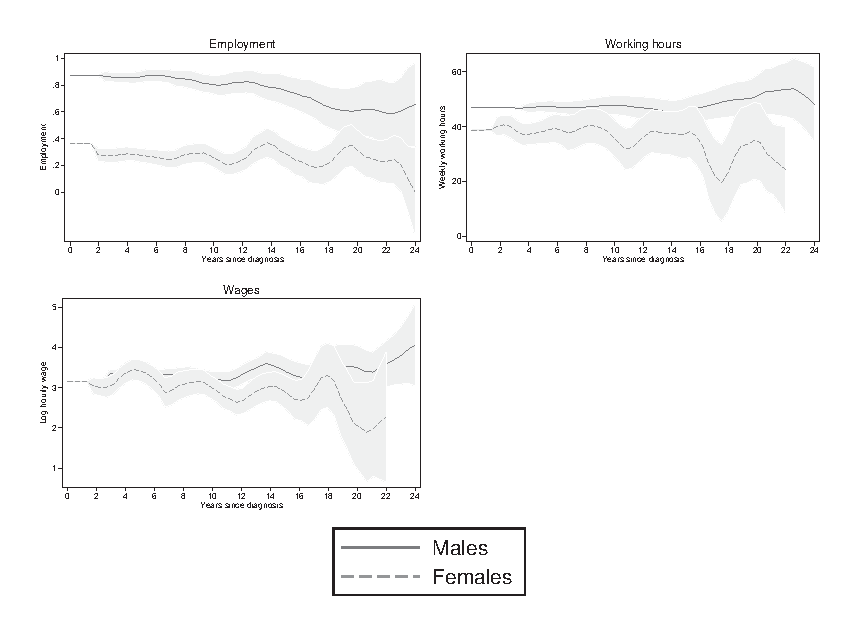
\includegraphics[width=\linewidth]{figures/lpoly_combined.eps}\\
\footnotesize{\textit{Notes} The dashed lines show 95\% confidence interval.}
\end{center}
\end{figure}

Tables \ref{tab:Self-reported-diabetes-duration_employ} and  \ref{tab:Self-reported-diabetes-duration_wage} present the estimation results for equations \ref{eq:duration_linear} and \ref{eq:splines}.

The results in Table \ref{tab:Self-reported-diabetes-duration_employ} panel A show that male employment probabilities fall every year in all models, with the biggest effects in the \ac{FE} model. For women, the coefficient shows a reduction of up to almost 1 percentage points per year in the \ac{FE} model, though its statistical significance is lower than in the \ac{OLS} models. 

\begin{table}[!ht]
\caption{\label{tab:Self-reported-diabetes-duration_employ}Relationship between self-reported years since diagnosis and employment probabilities using continuous duration and duration splines.}
\begin{center}
%\resizebox{\linewidth}{!}{%
\begin{adjustbox}{max width=\linewidth}
\begin{threeparttable}

{
\def\sym#1{\ifmmode^{#1}\else\(^{#1}\)\fi}
\begin{tabular}{l*{6}{S
S}}
\toprule
                &\multicolumn{3}{c}{Males}                               &\multicolumn{3}{c}{Females}                             \\\cmidrule(lr){2-4}\cmidrule(lr){5-7}
                &\multicolumn{1}{c}{(1)}&\multicolumn{1}{c}{(2)}&\multicolumn{1}{c}{(3)}&\multicolumn{1}{c}{(4)}&\multicolumn{1}{c}{(5)}&\multicolumn{1}{c}{(6)}\\
                  &\multicolumn{1}{c}{OLS}&\multicolumn{1}{c}{OLS}&\multicolumn{1}{c}{FE}&\multicolumn{1}{c}{OLS}&\multicolumn{1}{c}{OLS}&\multicolumn{1}{c}{FE}\\
                                &\multicolumn{1}{c}{(Wave 3)}&\multicolumn{1}{c}{(Pooled)}&\multicolumn{1}{c}{}&\multicolumn{1}{c}{(Wave 3)}&\multicolumn{1}{c}{(Pooled)}&\multicolumn{1}{c}{}\\
\midrule
\addlinespace
Panel A: linear &&&&&&\\
Diabetes duration &   -.008\sym{***}&    -.007\sym{***}&    -.017\sym{***}&    -.005\sym{***}&    -.004\sym{***}&    -.009\sym{*}  \\
                &   (.002)         &   (.002)         &   (.006)         &   (.002)         &   (.001)         &   (.005)         \\
                
\midrule
                Hausman test    &                  &                  &  153.024         &                  &                  &  200.073         \\
                \hspace*{10mm} p-value         &                  &                  &     .000         &                  &                  &     .000         \\
\midrule
\addlinespace
Panel B: splines&&&&&&\\
Diabetes duration &&&&&&\\
\hspace*{10mm}0--4&    -.007         &    -.007         &    -.026\sym{*}  &    -.010         &    -.015\sym{**} &    -.017         \\
                &   (.007)         &   (.006)         &   (.014)         &   (.007)         &   (.006)         &   (.016)         \\
\hspace*{10mm}5--11&     .000         &    -.003         &    -.003         &    -.004         &     .004         &    -.003         \\
                &   (.009)         &   (.006)         &   (.009)         &   (.008)         &   (.006)         &   (.008)         \\
\hspace*{10mm}12--20&  -.030\sym{**} &    -.017\sym{*}  &    -.029\sym{*}  &     .005         &    -.004         &    -.014         \\
                &   (.012)         &   (.010)         &   (.016)         &   (.008)         &   (.006)         &   (.011)         \\
\hspace*{10mm}> 20&     .011         &     .007         &    -.046\sym{*}  &    -.010\sym{*}  &    -.003         &    -.015         \\
                &   (.016)         &   (.014)         &   (.028)         &   (.006)         &   (.003)         &   (.018)         \\
\midrule
Hausman test    &                  &                  &  161.953         &                  &                  &  198.692         \\
\hspace*{10mm} p-value         &                  &                  &     .000         &                  &                  &     .000         \\
N               &     8217         &    16292         &    16292         &    10467         &    22407         &    22407         \\
\bottomrule
\end{tabular}
\begin{tablenotes}
\item \footnotesize \textit{Notes} The table presents the results of three estimation methods. Panel A presents the results of the linear specifications. Panel B presents the results of the non-linear specifications. Robust standard errors in parentheses. Other control variables: state dummies, urbanization dummies, education dummies, married dummy, number children < 6, wealth, age squared and calendar year dummies. The OLS and pooled OLS models additionally control for age. \sym{*} \(p<0.10\), \sym{**} \(p<0.05\), \sym{***} \(p<0.01\).
\end{tablenotes}
}
\end{threeparttable}
\end{adjustbox}
\end{center}
\end{table}

Panel B of Table \ref{tab:Self-reported-diabetes-duration_employ} shows the estimates when using a spline function. Focusing on the \ac{FE} results, the coefficients provide some evidence for an immediate effect of diabetes, which then levels off for some time after which it becomes stronger again. However, standard errors are quite large.

The results in Table \ref{tab:Self-reported-diabetes-duration_wage} indicate a reduction in female wages of about 7\% per year with diabetes in the \ac{FE} model. For men we find no consistent effect. The results of the non-linear specification in panel B of Table \ref{tab:Self-reported-diabetes-duration_wage} indicate that there may be a reduction in wages 5--11 years after the initial diagnosis for both men and women. We also find associations for women with more than 20 years of diabetes, but these estimates may be spurious due to the considerably reduced number of observations in this group.\footnote{There are only 9 and 3 observations for male and female wages with more than 20 years since diagnosis in wave 3, respectively, and 17 and 7 in the pooled sample, respectively. For male and female working hours there are 12 and 7 observations with more than 20 years since diagnosis in wave 3, respectively, and 20 and 12 for the pooled sample, respectively.} Interestingly, the reductions in wages found in the non-linear specification appear exactly at the time where employment probabilities are less affected. This could suggest that at this point reductions in productivity affect wages but are not so severe that they would cause job loss. 

\begin{table}[!ht]
\caption{\label{tab:Self-reported-diabetes-duration_wage}Relationship between self-reported years since diagnosis and log hourly wage using continuous duration and duration splines.}
\begin{center}
%\resizebox{\linewidth}{!}{%
\begin{adjustbox}{max width=\linewidth}
\begin{threeparttable}

{
\def\sym#1{\ifmmode^{#1}\else\(^{#1}\)\fi}
\begin{tabular}{l*{6}{S
S}}
\toprule
                &\multicolumn{3}{c}{Males}                               &\multicolumn{3}{c}{Females}                             \\\cmidrule(lr){2-4}\cmidrule(lr){5-7}
                &\multicolumn{1}{c}{(1)}&\multicolumn{1}{c}{(2)}&\multicolumn{1}{c}{(3)}&\multicolumn{1}{c}{(4)}&\multicolumn{1}{c}{(5)}&\multicolumn{1}{c}{(6)}\\
                &\multicolumn{1}{c}{OLS}&\multicolumn{1}{c}{OLS}&\multicolumn{1}{c}{FE}&\multicolumn{1}{c}{OLS}&\multicolumn{1}{c}{OLS}&\multicolumn{1}{c}{FE}\\
                 &\multicolumn{1}{c}{(wave 3)}&\multicolumn{1}{c}{(pooled)}&\multicolumn{1}{c}{}&\multicolumn{1}{c}{(wave 3)}&\multicolumn{1}{c}{(pooled)}&\multicolumn{1}{c}{}\\
\midrule
Panel A: linear &&&&&&\\
Diabetes duration&  .001         &     .010\sym{**} &    -.019         &    -.014\sym{*}  &    -.009         &    -.073\sym{**} \\
                &   (.006)         &   (.005)         &   (.018)         &   (.008)         &   (.008)         &   (.029)         \\
\midrule                
Hausman test    &                  &                  &  838.213         &                  &                  &   93.232         \\
\hspace*{10mm} p-value         &                  &                  &     .000         &                  &                  &     .000         \\                
\midrule
\addlinespace
Panel B: splines&&&&&&\\
Diabetes duration&&&&&&\\
\hspace*{10mm}0--4&      .034\sym{*}  &     .046\sym{***}&     .033         &     .027         &     .030         &     .015         \\
                &   (.017)         &   (.016)         &   (.055)         &   (.031)         &   (.026)         &   (.138)         \\
\hspace*{10mm}5--11&    -.041\sym{*}  &    -.037\sym{**} &    -.055\sym{*}  &    -.039         &    -.034         &    -.101\sym{*}  \\
                &   (.021)         &   (.018)         &   (.033)         &   (.030)         &   (.024)         &   (.056)         \\
\hspace*{10mm}12--20&      0.015         &     .044         &     .062         &    -.032         &    -.071\sym{*}  &    -.051         \\
                &   (.033)         &   (.029)         &   (.056)         &   (.042)         &   (.039)         &   (.047)         \\
\hspace*{10mm}> 20&     .053         &     .014         &    -.111         &    -.007         &     .041\sym{***}&    -.204\sym{***}\\
                &   (.054)         &   (.040)         &   (.104)         &   (.028)         &   (.015)         &   (.053)         \\
\midrule
Hausman test    &                  &                  & 1037.290         &                  &                  &   96.266         \\
\hspace*{10mm} p-value         &                  &                  &     .000         &                  &                  &     .000         \\
N               &     5509         &    10767         &    10767         &     2874         &     5741         &     5741         \\
\bottomrule
\end{tabular}
\begin{tablenotes}
\item \footnotesize \textit{Notes} The table presents the results of three estimation methods for log hourly wages. Panel A presents the results of the linear specifications. Panel B presents the results of the non-linear specifications. Robust standard errors in parentheses. Other control variables: state dummies, urbanization dummies, education dummies, married dummy, number children < 6, wealth, age squared, calendar year dummies, type of work (agricultural and self employed with dependent non-agricultural wage employment as the base) and health insurance status. The OLS and pooled OLS models additionally control for age. \sym{*} \(p<0.10\), \sym{**} \(p<0.05\), \sym{***} \(p<0.01\).
\end{tablenotes}
}
\end{threeparttable}
\end{adjustbox}
\end{center}
\end{table}

The estimation results in Table \ref{tab:Self-reported-diabetes-duration_hours} indicate that there appears to be no consistent relationship between working hours and time since being diagnosed with diabetes, neither for men nor for women.


Taken together, these results suggest a fairly constant decrease in the probability of employment for both men and women and in earnings for women, which contrast with estimates for the USA \parencite{Minor2013}, where no such relationship is observed.  \textcite{Minor2013} finds a reduction in employment probabilities of 82 percentage points for females after 11 to 15 years and a reduction of 60 percentage points for males after 2-5 years, indicating very large employment penalties, in particular in comparison to our results for Mexico. However, the non-linear results we presented are not directly comparable to these estimates as Minor used pooled cross-sectional data, constructed dummy variables instead of splines and used different duration groups. When we use a similar model to \textcite{Minor2013}  the results confirm that the employment effects are substantially less negative in Mexico than in US. For men they reduce with 6-12\% in the first 2 and 4 years respectively---depending on the specification used, and some increase in the following years. We find no immediate effect of diagnosis for women, but effects do emerge after about 2 years and tend to increase somewhat over time.\footnote{Following \textcite{Minor2013} we find a significant reduction in employment probabilities throughout, regardless of whether we use our duration groups to construct the dummies or the duration groups used by \textcite{Minor2013}.} 

The increasing adverse effects of diabetes over time are plausible in that as time lived with diabetes evolves, complications associated with diabetes tend to become more frequent and more severe \parencite{Adler2003}. Looking at wages as our labor market outcome, we uncover some adverse effects for females, indicating a sizeable reduction with time since diagnosis.


\begin{table}[p]
\caption{\label{tab:Self-reported-diabetes-duration_hours}Relationship between self-reported years since diagnosis and weekly working hours using continuous duration and duration splines.}
\begin{center}
%\resizebox{\linewidth}{!}{%
\begin{adjustbox}{max width=\linewidth}
\begin{threeparttable}
{
\def\sym#1{\ifmmode^{#1}\else\(^{#1}\)\fi}
\begin{tabular}{l*{6}{S
S}}
\toprule
                &\multicolumn{3}{c}{Males}                               &\multicolumn{3}{c}{Females}                             \\\cmidrule(lr){2-4}\cmidrule(lr){5-7}
                &\multicolumn{1}{c}{(1)}&\multicolumn{1}{c}{(2)}&\multicolumn{1}{c}{(3)}&\multicolumn{1}{c}{(4)}&\multicolumn{1}{c}{(5)}&\multicolumn{1}{c}{(6)}\\
                &\multicolumn{1}{c}{OLS}&\multicolumn{1}{c}{OLS}&\multicolumn{1}{c}{FE}&\multicolumn{1}{c}{OLS}&\multicolumn{1}{c}{OLS}&\multicolumn{1}{c}{FE}\\
                 &\multicolumn{1}{c}{(wave 3)}&\multicolumn{1}{c}{(pooled)}&\multicolumn{1}{c}{}&\multicolumn{1}{c}{(wave 3)}&\multicolumn{1}{c}{(pooled)}&\multicolumn{1}{c}{}\\
\midrule
Panel A: linear &&&&&&\\
Diabetes duration & .069         &     .048         &     .181         &    -.020         &    -.124         &     .208         \\
                &   (.124)         &   (.102)         &   (.330)         &   (.187)         &   (.127)         &   (.652)         \\
\midrule
Hausman test    &                  &                  &  704.904         &                  &                  &  107.709         \\
\hspace*{10mm} p-value         &                  &                  &     .000         &                  &                  &     .000         \\
\midrule
\addlinespace
Panel B: splines &&&&&&\\
Diabetes duration &&&&&&\\
\hspace*{10mm}0--4&      -.033         &    -.233         &     .709         &     .739         &     .470         &    2.014         \\
                &   (.421)         &   (.325)         &   (.938)         &   (.645)         &   (.586)         &  (2.947)         \\
\hspace*{10mm}5--11&  .269         &     .338         &    -.218         &    -.410         &    -.479         &    -.508         \\
                &   (.539)         &   (.399)         &   (.568)         &   (.728)         &   (.553)         &  (1.020)         \\
\hspace*{10mm}12--20&    .209         &     .137         &     .698         &    -.164         &    -.051         &    -.402         \\
                &   (.730)         &   (.538)         &   (.945)         &   (.995)         &   (.700)         &  (1.207)         \\
\hspace*{10mm}> 20&  -1.300         &    -.768         &     .039         &    -.499         &    -.418         &    8.117\sym{***}\\
                &   (.944)         &   (.930)         &  (2.184)         &   (.930)         &   (.305)         &  (1.612)         \\
\midrule
Hausman test    &                  &                  &  724.225         &                  &                  &  112.627         \\
\hspace*{10mm} p-value         &                  &                  &     .000         &                  &                  &     .000         \\
N               &     6807         &    13581         &    13581         &     3591         &     7383         &     7383         \\
\bottomrule
\end{tabular}
\begin{tablenotes}
\item \footnotesize \textit{Notes} The table presents the results of three estimation methods for weekly working hours. Panel A presents the results of the linear specifications. Panel B presents the results of the non-linear specifications. Robust standard errors in parentheses. Other control variables: state dummies, urbanization dummies, education dummies, married dummy, number children < 6, wealth, age squared, calendar year dummies, type of work (agricultural and self employed with dependent non-agricultural wage employment as the base) and health insurance status. The OLS and pooled OLS models additionally control for age. \sym{*} \(p<0.10\), \sym{**} \(p<0.05\), \sym{***} \(p<0.01\).
\end{tablenotes}
}
\end{threeparttable}
\end{adjustbox}
\end{center}
\end{table}

\FloatBarrier

\subsection{Cross-sectional biomarker analysis}


Table \ref{tab:Biomarker_observations} presents a cross tabulation of self-reported diabetes and biomarker results, indicating that 27\% of the sample have \ac{HbA1c} levels indicative of diabetes and 81\% of those self-reporting a diabetes diagnosis also have \ac{HbA1c} levels equal to or above the diabetes threshold. The cell percentages in the table underline the large proportion of false negatives (18\%). The 3\% with self-reported diabetes but biomarker levels below the diabetes threshold could be interpreted as false positives, however, likely a large proportion has received a diabetes diagnosis but has achieved blood glucose levels below the diabetes threshold thanks to treatment and lifestyle changes. Of the respondents who tested positive for diabetes according to the biomarker analysis, 32\% self-report a diagnosis, while 68\% do not. There are no considerable differences to the presented proportions in Table \ref{tab:Biomarker_observations} if we look at men and women separately and we therefore do not show these results here. 


\begin{table}[ht]
\caption{\label{tab:Biomarker_observations}Number of observations with diabetes (HbA1c $\geq 6.5\%$) and self-reported diabetes.}
\begin{center}
\begin{adjustbox}{max width=\linewidth}
\begin{threeparttable}
{
\def\sym#1{\ifmmode^{#1}\else\(^{#1}\)\fi}
\begin{tabular}{l*{3}{S S}}
\toprule
            &\multicolumn{1}{c}{$HbA1c < 6.5\%$}&\multicolumn{1}{c}{HbA1c $\geq 6.5\%$}&\multicolumn{1}{c}{Total}\\
\midrule
No self-reported diabetes (N) & 4544 & 1181 & 5725 &  \\
\hspace*{10mm}Row  \% & 79\% & 21\% & 100\% &  \\
\hspace*{10mm}Column \% & 97\% & 68\% & 89\% &  \\
\hspace*{10mm}Cell \% & 71\% & 18\% & z & \\
Self-reported diabetes (N) & 129 & 554 & 683 &  \\
\hspace*{10mm}Row \%  & 19\% & 81\% & 100\% &  \\
\hspace*{10mm}Column \% & 3\% & 32\% & 11\% &  \\
\hspace*{10mm}Cell \% & 2\% & 9\% & z & \\
Total (N) & 4673 & 1735 & 6408 &  \\
\hspace*{10mm}Row \% & 73\% & 27\% & 100\% &  \\
\hspace*{10mm}Column \%  & 100\% & 100\% & 100\% &  \\
\hspace*{10mm}Cell \% & x & y & z & \\  
\bottomrule
\end{tabular}
\begin{tablenotes}
\item
\end{tablenotes}
}
\end{threeparttable}
\end{adjustbox}
\end{center}
\end{table}

Table \ref{tab:Biomarker_results} presents the results from estimating equations \ref{eq:diab_sr}, \ref{eq:diab} and \ref{eq:diab_ud}.  
The results in columns 1 and 2 of Table \ref{tab:Biomarker_results} show that the earlier longitudinal results using self-reported diabetes are robust for the biomarker sample. The coefficients in column 3 and 4 indicate that the relationship becomes much weaker when using diabetes defined by the biomarker instead of self-reported diabetes.\footnote{We also created a dummy variable that additionally to measured diabetes accounted for those with a self-reported diabetes diagnosis but biomarker levels below the diabetes threshold. This is of interest because those who suffer from diabetes but manage to control their sugar levels may obtain test results outside the diabetes range.  If one would choose to believe there is no misreporting, this can be seen as representing the entire diabetes population. The coefficients and their statistical significance are only marginally different to those presented in columns 3 and 4 of Table 8, which is why we do not present them here.} In columns 5 and 6 of Table \ref{tab:Biomarker_results}, obtained from estimating equations \ref{eq:diab_ud}, the coefficient for the biomarker diabetes population now reflects the effect of undiagnosed diabetes, as the regression includes a control for self-reported diabetes, revealing that labor outcomes are not lower for those with undiagnosed diabetes. 

\begin{table}[h]
\caption{\label{tab:Biomarker_results}Biomarker results}
\begin{center}
\begin{adjustbox}{max width=\linewidth}
\begin{threeparttable}
{
\def\sym#1{\ifmmode^{#1}\else\(^{#1}\)\fi}
\begin{tabular}{l*{6}{S
S}}
\toprule
                &\multicolumn{1}{c}{(1)}&\multicolumn{1}{c}{(2)}&\multicolumn{1}{c}{(3)}&\multicolumn{1}{c}{(4)}&\multicolumn{1}{c}{(5)}&\multicolumn{1}{c}{(6)}\\
                &\multicolumn{1}{c}{Males}&\multicolumn{1}{c}{Females}&\multicolumn{1}{c}{Males}&\multicolumn{1}{c}{Females}&\multicolumn{1}{c}{Males}&\multicolumn{1}{c}{Females}\\
\midrule
\multicolumn{7}{l}{\hspace*{10mm}\textbf{Dependent variable: Employment}} \\
Self-reported diabetes&   -.051\sym{**} &    -.044\sym{*}  &                  &                  &    -.053\sym{**} &    -.032         \\
                &   (.026)         &   (.023)         &                  &                  &   (.026)         &   (.026)         \\
HbA1c $\geq$ 6.5&                  &                  &    -.012         &    -.031\sym{*}  &     .003         &    -.022         \\
                &                  &                  &   (.016)         &   (.018)         &   (.017)         &   (.019)         \\
\midrule
N               &\multicolumn{1}{S}{2785}         &\multicolumn{1}{S}{3623}         &\multicolumn{1}{S}{2785}         &\multicolumn{1}{S}{3623}         &\multicolumn{1}{S}{2785}         &\multicolumn{1}{S}{3623}         \\
\midrule
\multicolumn{7}{l}{\hspace*{10mm}\textbf{Dependent variable: Log hourly wages}} \\ 
\addlinespace
Self-reported diabetes&    -.010         &    -.040         &                  &                  &    -.006         &    -.010         \\
                &   (.065)         &   (.113)         &                  &                  &   (.078)         &   (.119)         \\
HbA1c $\geq$ 6.5&                  &                  &    -.007         &    -.057         &    -.006         &    -.055         \\
                &                  &                  &   (.044)         &   (.070)         &   (.049)         &   (.075)         \\
\midrule
N               &\multicolumn{1}{S}{1803}         &\multicolumn{1}{S}{884}         &\multicolumn{1}{S}{1803}         &\multicolumn{1}{S}{884}         &\multicolumn{1}{S}{1803}         &\multicolumn{1}{S}{884}         \\
\midrule
\multicolumn{7}{l}{\hspace*{10mm}\textbf{Dependent variable: Weekly working hours}} \\ 
\addlinespace
Self-reported diabetes&   -.293         &    -.751         &                  &                  &    -.286         &   -1.566         \\
                &  (1.305)         &  (2.178)         &                  &                  &  (1.419)         &  (2.351)         \\
HbA1c $\geq$ 6.5&                  &                  &    -.088         &    1.153         &    -.012         &    1.525         \\
                &                  &                  &   (.844)         &  (1.462)         &   (.925)         &  (1.565)         \\
\bottomrule
\end{tabular}
\begin{tablenotes}
\item \footnotesize \textit{Notes} Community level fixed effects. Robust standard errors in parentheses. Other control variables: age, age squared, state dummies, urbanization dummies, education dummies, married dummy, number children < 6 and wealth. Calender year dummies are included as data collection for the third wave was stretched out over several years. The wage and working hour models additionally control for type of work (agricultural and self employed with non-agricultural wage employment as the base) and for health insurance status. \sym{*} \(p<0.10\), \sym{**} \(p<0.05\), \sym{***} \(p<0.01\).
\end{tablenotes}
}
\end{threeparttable}
\end{adjustbox}
\end{center}
\end{table}

To explore whether this stems from selection into the diagnosed population of those with a more severe diabetes---proxied by higher \ac{HbA1c} levels---and a therefore higher risk to lose their job,  we test whether those with self-reported diabetes have higher levels of \ac{HbA1c} than those who were not diagnosed, using a t-test, and find that they do.\footnote{Men: Self-reported diabetes \ac{HbA1c} of 9.0\% vs 8.5\% in those undiagnosed (p < 0.01); Women: Self-reported diabetes \ac{HbA1c} of 8.9\% vs 8.7\% in those undiagnosed (p < 0.05).} We then extend the model to take into account the severity of diabetes more explicitly, using the measured HbA1c levels. If current severity would be related to labour outcomes and explain the difference in effects of self-reported and undiagnosed diabetes, one would expect (i) that those with higher \ac{HbA1c} levels have lower probability of employment, and (ii) that the inclusion of diabetes severity weakens the coefficient of self-reported.  To investigate this, we replace the indicator variable for diabetes with a variable that takes the value zero for levels below and the actual value of \ac{HbA1c} for those above the diabetes threshold. The results in Table \ref{tab:Diagnosed_undiagnosed_robust}, panel A do not find a consistent relationship between increased \ac{HbA1c} levels and the probability of employment, suggesting that disease severity may not explain the different employment effects of diabetes. 

Secondly, to assess whether the differences in effect are driven by differences in subjective health, we include additional controls for self-reported health. The results are reported in Table \ref{tab:Diagnosed_undiagnosed_robust}, panel B, and indicate that the relationship between employment and self-reported diabetes becomes weaker, resulting in reduced difference between self-reported and undiagnosed diabetes. For women, the point estimates for self-reported diabetes and undiagnosed diabetes are now virtually of the same size, suggesting that differences in general health drive the above results, though the difference was not very big to begin with. For men, it appears differences in health between the two groups play a role, however, other unobserved factors are still important.

Thirdly, instead of controlling for subjective health we include a battery of indicators for other chronic diseases that are often related to diabetes. In detail, we control for overweight and obesity (based on anthropometrically measured \ac{BMI}) and self-reports of a diagnosis of hypertension and heart disease. If those diagnosed with diabetes are more likely to experience adverse employment outcomes because they are more likely to suffer from one of these diseases, then accounting for them should lead to a sizeable reduction in the coefficient of self-reported diabetes. In line with the results in panel B, we find a reduction in the coefficient for self-reported diabetes in both men and women, though the reduction here is much bigger for men than for women. Having had a diagnosis of heart disease is significantly associated with lower employment probabilities for men, and overall the coefficient for self-reported diabetes in men is reduced by about one percentage point after the inclusion of these diabetes related diseases.\footnote{Further analysis indicates that the reductions in the diabetes coefficient for men appear after the inclusion of heart disease as well as hypertension, while ovwerweight and obesity play a minor role.}

\begin{table}[h]
\caption{\label{tab:Diagnosed_undiagnosed_robust}Self-reported diabetes, biomarkers, diabetes severity and self-reported health and their association with labor outcomes}
\begin{center}
\begin{adjustbox}{max width=\linewidth} 
\begin{threeparttable} 
{
\def\sym#1{\ifmmode^{#1}\else\(^{#1}\)\fi}
\begin{tabular}{l*{6}{S
S}}
\toprule
                &\multicolumn{2}{c}{Employment}       &\multicolumn{2}{c}{Log hourly wages} &\multicolumn{2}{c}{Weekly working hours}\\\cmidrule(lr){2-3}\cmidrule(lr){4-5}\cmidrule(lr){6-7}
                &\multicolumn{1}{c}{(1)}&\multicolumn{1}{c}{(2)}&\multicolumn{1}{c}{(3)}&\multicolumn{1}{c}{(4)}&\multicolumn{1}{c}{(5)}&\multicolumn{1}{c}{(6)}\\
                &\multicolumn{1}{c}{Males}&\multicolumn{1}{c}{Females}&\multicolumn{1}{c}{Males}&\multicolumn{1}{c}{Females}&\multicolumn{1}{c}{Males}&\multicolumn{1}{c}{Females}\\
\midrule
\multicolumn{6}{l}{\hspace*{10mm}\textbf{Panel A (HbA1c levels)}}\\
Self-reported diabetes&     -.057\sym{*}  &    -.027         &    -.004         &    -.009         &    -.101         &   -1.607         \\
                &   (.031)         &   (.025)         &   (.069)         &   (.113)         &  (1.370)         &  (2.363)    \\     
HbA1c (if HbA1c $\geq 6.5\%$)  &     .001         &    -.003         &    -.001         &    -.005         &    -.030         &     .151         \\
                &   (.002)         &   (.002)         &   (.005)         &   (.008)         &   (.103)         &   (.172)         \\
\midrule
N               &     2785         &     3623         &     1803         &      884         &     2302         &     1144         \\
\midrule
\multicolumn{6}{l}{\hspace*{10mm}\textbf{Panel B (other chronic diseases)}}\\
Self-reported diabetes=1&    -.044\sym{*}  &    -.029         &     .005         &     .053         &    -.131         &   -1.411         \\
                &   (.026)         &   (.027)         &   (.079)         &   (.120)         &  (1.438)         &  (2.385)         \\
HbA1c $\geq 6.5\%$=1&     .001         &    -.021         &    -.010         &    -.037         &    -.077         &    1.382         \\
                &   (.017)         &   (.019)         &   (.049)         &   (.076)         &   (.927)         &  (1.572)         \\

Overweight &     .021         &    -.003         &     .093\sym{**} &     .034         &    -.225         &   -1.520         \\
                &   (.016)         &   (.020)         &   (.046)         &   (.072)         &   (.874)         &  (1.528)         \\
Obese&     .022         &    -.030         &     .086         &    -.026         &     .895         &    -.385         \\
                &   (.019)         &   (.020)         &   (.053)         &   (.075)         &  (1.003)         &  (1.578)         \\
Hypertension    &    -.035         &    -.020         &    -.106         &    -.089         &    -.447         &   -1.828         \\
                &   (.025)         &   (.022)         &   (.072)         &   (.089)         &  (1.370)         &  (1.854)         \\
Heart disease   &    -.165\sym{***}&    -.045         &     .060         &    -.039         &   -2.640         &   -5.430         \\
                &   (.059)         &   (.050)         &   (.179)         &   (.215)         &  (3.659)         &  (4.854)         \\
\midrule
N               &     2785         &     3621         &     1803         &      883         &     2302         &     1143         \\
\midrule
\multicolumn{6}{l}{\hspace*{10mm}\textbf{Panel C (self-reported health)}}\\  
Self-reported diabetes&   -.036         &    -.023         &     .002         &     .060         &     .123         &   -2.191         \\
                &   (.026)         &   (.027)         &   (.079)         &   (.121)         &  (1.433)         &  (2.386)         \\        
Hba1c $\geq 6.5\%$&       .003         &    -.023         &    -.004         &    -.051         &    -.066         &    1.829         \\
                &   (.017)         &   (.019)         &   (.049)         &   (.075)         &   (.926)         &  (1.569)         \\
\multicolumn{6}{l}{Self-reported health status}\\
\hspace*{10mm}good&    .023         &     .057\sym{*}  &     .061         &    -.115         &   -1.131         &    3.521         \\
                &   (.025)         &   (.034)         &   (.074)         &   (.124)         &  (1.376)         &  (2.499)         \\
\hspace*{10mm}fair&    -.007         &     .006         &     .025         &    -.157         &   -1.606         &    4.646\sym{*}  \\
                &   (.026)         &   (.034)         &   (.076)         &   (.128)         &  (1.424)         &  (2.607)         \\
\hspace*{10mm}bad &    -.127\sym{***}&    -.024         &    -.016         &    -.371\sym{*}  &   -6.190\sym{**} &    6.918\sym{*}  \\
                &   (.043)         &   (.046)         &   (.135)         &   (.189)         &  (2.521)         &  (3.858)         \\
\hspace*{10mm}very bad&    -.165         &     .117         &    -.331         &     .316         &   -1.869         &  -17.400\sym{*}  \\
                &   (.110)         &   (.116)         &   (.300)         &   (.439)         &  (6.433)         &  (9.005)         \\
\midrule
N               &\multicolumn{1}{S}{2785}         &\multicolumn{1}{S}{3621}         &\multicolumn{1}{S}{1803}         &\multicolumn{1}{S}{883}         &\multicolumn{1}{S}{2302}         &\multicolumn{1}{S}{1143}         \\
\bottomrule
\end{tabular}
\begin{tablenotes}
\item \footnotesize \textit{Notes} Community level fixed effects. Robust standard errors in parentheses. Other control variables: age, age squared, state dummies, urbanization dummies, education dummies, married dummy, number children < 6 and wealth. Calender year dummies are included as data collection for the third wave was stretched out over several years. The wage and working hour models additionally control for type of work (agricultural and self employed with non-agricultural wage employment as the base) and for health insurance status. \sym{*} \(p<0.10\), \sym{**} \(p<0.05\), \sym{***} \(p<0.01\).
\end{tablenotes}
}
\end{threeparttable}
\end{adjustbox}
\end{center}
\end{table}

It is interesting to contrast these results with those obtained from \textcite{BrownIII2011}, one of two other studies that uses biomarker data. Using data for a Mexican American population the study finds that once diabetes is diagnosed blood glucose levels themselves have little effect on labour outcomes. This is not surprising given that HbA1c levels only provide a picture of blood glucose levels over the last three months. They therefore may not be representative of blood glucose levels in the years before and after the diabetes diagnosis which ultimately determine how soon complications appear and how severe they will be.

In the same vein, \parencite{Minor2015} find for a USA population that people with undiagnosed diabetes experience smaller employment penalties than those self-reporting the condition. The study finds, however, much bigger effects than we do when estimating the impact of biometrically measured diabetes. One possible explanation for the difference is that the undiagnosed population made up a much smaller share of the overall diabetes population compared to our context, and is therefore likely to have a distinct profile.
\FloatBarrier


\section{\label{sec:cha_4_conclusion}Conclusion}

Diabetes is now one of the most common chronic diseases in middle- and high-income countries, with the potential to severely impact the health and economic well-being of those affected. Yet rigorous evidence on the economic consequences for these countries remains scarce.

To address key methodological challenges this paper uses rich longitudinal panel data from Mexico that also contain biomarker data. The biomarker data confirm the alarming levels of clinically tested diabetes, 27\%, and indicate that a large proportion of these (68\% of those with diabetes or 18\% of the population) are unaware that they have the condition. 

The paper finds evidence for adverse effects of self-reported diabetes on the probability of being employed, but not on wages or hours worked, using fixed effects estimation.  Considering different types of work, the relationship between self-reported diabetes, and wages and hours worked remains weak, but the results also suggest occupational selection with women with self-reported diabetes less likely to work in agriculture.  A dynamic analysis finds that the employment probability falls gradually over the years after having been diagnosed with this chronic condition.  

Making use of the biomarker data allows us to both test reporting error and the effects of undiagnosed diabetes. The results confirm the large proportion that is unaware of the condition.  We contrast impact of self-reported and tested diabetes, and find that it is similar for women but not for men.  Combined results suggest lower employment for the diagnosed, especially for men, while there is no employment effect for undiagnosed men or women.  This lack of employment effect for undiagnosed men seems to stem from better general health rather than less severe diabetes. The results highlight both the importance of the economic impact of diabetes, and the need to take into account (especially female) undiagnosed patients, especially for women. 

The second part of our results indicates that only relying on self-reported diabetes can lead to an overestimation of the relationship between diabetes and labor outcomes. We find that a negative relationship only exists for those with self-reported, but not for those with undiagnosed diabetes. This perhaps surprising, notable difference, is at least mediated by the subjective health status being worse for those self-reporting compared to the undiagnosed. Current disease severity, as proxied by \ac{HbA1c} levels, does not appear to play an important role in this context.

Our findings bear several implications. First, when interpreting labor market impact estimates relying on self-reported diabetes, one cannot assume that the results extend to those with undiagnosed diabetes. However, simply merging self-reported and undiagnosed in one diabetes category may not be ideal either, as doing so will fail to account for the heterogeneity between the groups in terms of health information, their actual time of living with diabetes and consequently their subjective as well as true health status, leading to a potentially important loss of information. By contrast, accounting for both groups separately acknowledging their inherent differences, allows to gain information about the distribution of the economic burden across the two groups.

Our results add further weight to the case for reducing the incidence and progression of diabetes. On top of the well-documented health benefits, it appears there are considerable gains to be had by increasing the productive lifespan of people. This is of particular importance in \acl{LMICs}, where parental health shocks, related job loss and increasing health expenditures can have repercussions across the entire household. Other family members, including children, may be forced to increase their labor supply and to reduce non-health expenditures in order to prevent a deterioration of the household's economic situation. This can lead to forgone investments into child education, showcasing the potential for adverse long-term effects of health shocks due to diabetes \parencite{Bratti2014}. Moreover, the large proportion of previously undiagnosed cases indicates that diagnosis---at least in Mexico---still happens too late or not at all. This reduces the possibilities to prevent complications via treatment and self-management, consequently increasing the risk of severe complications appearing earlier. Hence, much of the health and economic burden may be prevented by earlier diagnosis and, given the generally limited success in achieving good blood-glucose control in Mexico, better treatment of those already diagnosed with diabetes. Ultimately of course, there will be a need to invest in the prevention of diabetes. Taxation of sugar sweetened beverages may be one promising way forward \parencite{Colchero2016}, though the long-term effects remain to be demonstrated. Further, considering the double-disease burden of non-communicable and communicable diseases and malnutrition in many \acl{LMICs}, investments in maternal and child health may not only reduce the current disease burden but would likely reduce the future incidence of diabetes, given the established links between early life heath status and later life incidence of diabetes and other chronic diseases \parencite{Sotomayor2013,Hanson2012,Li2010b}.  

Our results indicate a significant economic burden of diabetes and it is unlikely that it will be reduced in the near future given that diabetes has started appearing at an increasingly younger age in many \ac{LMICs}, causing people to live with the disease for larger parts of their productive lifespan, possibly exacerbating the economic effects of reduced employment due to diabetes \parencite{Hu2011,Villalpando2010}. Therefore, population level measures as well as efforts to improve early-life health are needed to prevent a further increase in diabetes, as is a better integration of diabetes care in the existing health system will be needed to reduce its burden now and in the future.

\begin{appendix}
\clearpage


\part*{\label{part:Appendix}Appendix}

\section{\label{sec:Appendix}Strategies to deal with inconsistent self-reporting over time}

Reporting error can pose a considerable challenge in the use of self-reported data. Fortunately, the \ac{MxFLS} data provides several possibilities to assess the amount of misreporting and apply corrections before estimating the labor market effects of diabetes. In what follows we describe how we deal with inconsistencies in self-reported diabetes over time.


Throughout the surveys, self-reported diabetes was measured by the question 'Have you ever been diagnosed by diabetes'. If they answered 'yes', they were asked if they received treatment for diabetes and the type of treatment they received.

One of the key advantages of panel data is the repeated measurement which results in more than one data point, which allows to uncover inconsistencies for cases with multiple observations. Very little is known about inconsistencies in self-reported diabetes over time. However, \textcite{Zajacova2010} assess the consistency of a self-reported cancer diagnosis over time in the USA. The study found that 30\% of those who had reported a cancer diagnosis at an earlier point failed to report the diagnosis at a later point in time. A more recent diagnosis was found to be reported with greater consistency possibly due to increasing recall problems as time since diagnosis passes.

Assessing the data we use, we also find inconsistencies in the diabetes self-reports across the three waves, with between 10--20\% of those reporting diabetes in one wave not doing so in one of the subsequent waves. To improve the validity of diabetes self-reports, we are interested in reducing the amount of reporting inconsistencies.

As discussed at the end of section \ref{sec:Data}, for diabetes for diabetes, the main concern with mismeasurement is related to false negatives. False positives are deemed less of a problem since there seems limited incentives to report diabetes when one does not have it – although we cannot exclude this.  A study from China finds that the vast majority (98\%) of those who self-report diabetes are tested positive for diabetes, while only a minority  of those who are tested positive for diabetes (40\%), actually self-report the disease \parencite{Yuan2015}.  Our data shows a similar pattern, with a negligible proportion (3\%) of the respondents who are tested negative self-reporting to suffer from diabetes, while the majority of those who are tested positive (68\%) do not self-report suffering from diabetes.

We used the above information to infer the "true" diabetes status for those with inconsistent reports. For respondents present in all three waves, we corrected inconsistencies as reported in Table \ref{tab:Inconsistencies}. We assumed that if diabetes was reported only once in the first two waves (either in 2002 or 2005) and then not reported again in the ensuing waves, this diabetes report was likely to be false (see lines 3 and 4 in Table \ref{tab:Inconsistencies}) and that the person never had received a diagnosis. If a diabetes diagnosis was however reported in two of the three waves (in 2002 and 2009 but not 2005, or in 2002 and 2005 but not in 2009) we assumed that the respondent had diabetes in all three waves (see lines 1 and 2 in Table \ref{tab:Inconsistencies}). For those cases where we only had information from two waves, we assumed that if a diabetes diagnosis had been reported in a prior wave they also had diabetes in the ensuing wave, even if it was not reported in the latter (see lines 5 and 6 in Table \ref{tab:Inconsistencies}). This relies on the assumption that diabetes does not go away: once one has had diabetes, it can be managed to keep blood sugar levels outside the diabetes range, but the condition cannot be abolished.


\begin{table}[h!]
\caption{\label{tab:Inconsistencies}Inconsistencies in diabetes self-report in MxFLS.}
\begin{center}
\begin{adjustbox}{max width=\linewidth} 
\begin{tabular}{lllc}
\hline 
 &Inconsistency  & Assumption  & Number of observations replaced\tabularnewline
\hline 
1 &Diabetes self-report only in 2002, but not in 2005 and 2009  & Has no diabetes in 2002 either  & 66\tabularnewline
2 &Diabetes self-report only in 2005, but not in 2002 and 2009  & Has no diabetes in 2005 either  & 52\tabularnewline
3 &Diabetes self-report in 2002, 2005 but not in 2009  & Has diabetes in 2009 as well  & 19\tabularnewline
4 &Diabetes self-report in 2002, 2009 but not in 2005  & Has diabetes in 2005 as well  & 63\tabularnewline
5 &Diabetes self-report in 2002, but not in 2005. Not in survey in 2009  & Has diabetes in 2005 as well  & 44\tabularnewline
6 &Diabetes self-report in 2005, but not in 2009. Not in survey in 2002  & Has diabetes in 2009 as well  & 23\tabularnewline
\end{tabular}
\end{adjustbox}
\end{center}
\end{table}

We then test if those respondents we categorized as not having a diabetes diagnosis based on above rules are actually more likely to not have diabetes, using the biomarker data from wave 3. Of those with inconsistencies in their diabetes self-reports, 95 were present in the biomarker sample (46 with two self-reports (from lines 3 and 4 in Table \ref{tab:Inconsistencies}) and 49 with one self-report of diabetes (from lines 1 and 2 in Table \ref{tab:Inconsistencies})). Figure \ref{fig:kdens_inconsistency_hba1c} illustrates the difference between both groups and suggests that indeed those with two self-reports of diabetes are much more likely to have \ac{HbA1c} values above the diabetes threshold. A t-test comparing the mean \ac{HbA1c} for the two groups indicates that those with two self-reports also have significantly (p<0.001) higher \ac{HbA1c} levels than those with only one self-report of diabetes (9.7\% vs. 7.1\%). Further, of those with one self-report, for only 30\% the \ac{HbA1c}$\geq6.5$\% compared to 87\% of those with two self-reports. Based on these results it appears that we did minimize misclassification of people into diabetes or no-diabetes. 

Alternatively we also test if using an alternative strategy, i.e. assuming that everybody who reported  a diabetes diagnosis once had diabetes in any later wave, would lead to different estimation results. We do not find this to be the case and find only minor differences in the point estimates of the coefficients (results available on request). 

\begin{figure}[h!]
\caption{\label{fig:kdens_inconsistency_hba1c}Kernel density of HbA1c values for those with one inconsistent and two inconsistent reports.}%
\begin{center}
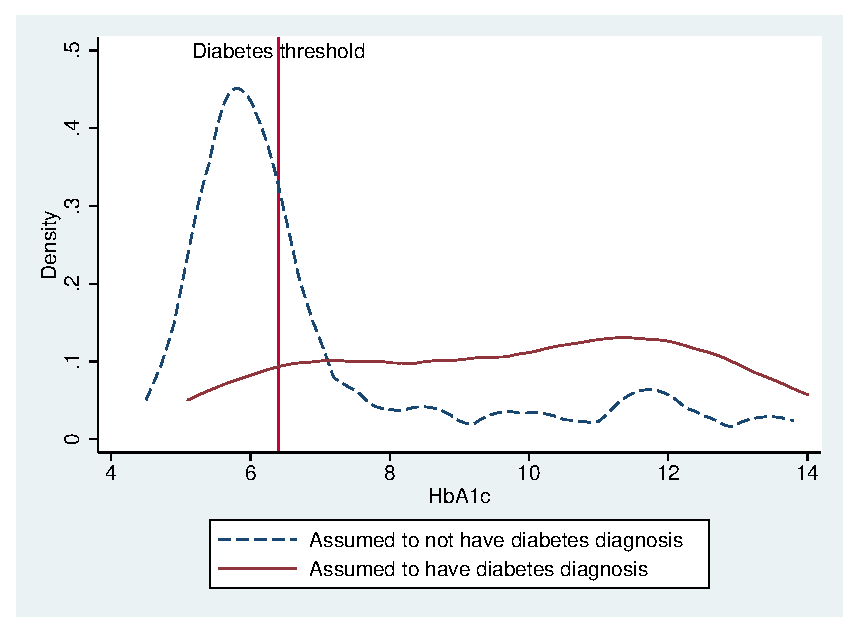
\includegraphics[width=.5\linewidth]{figures/kdensity_hba1c_inconsist.eps}\\
\end{center}
\end{figure}





\end{appendix}

\subsection*{Acknowledgements}

We are grateful to the participants at the European Health Economics Association PhD-Supervisor conference September 2015 in Paris, the Health, Education and Labor Market Outcomes Workshop at the WifOR Institute in October 2015 in Darmstadt, Germany, seminar participants at the Centre for Health Economics at York University, and Max Bachmann for helpful comments.




%\noindent \bibliographystyle{elsarticle-harv} 

\printbibliography

%\bibliography{/home/till/Dokumente/BibTex/Second_Mexico_paper-Article}
\end{document}

